\documentclass{beamer}
\usecolortheme{wolverine}

% math stuff
\usepackage{amsmath}
\usepackage{amsthm}
\usepackage{amssymb}
\usepackage{xcolor}

\usepackage{float}
\usepackage{subcaption}

% to insert images
\usepackage{graphicx}

% to correctly insert stressed characters
\usepackage[T1]{fontenc}
\usepackage[utf8]{inputenc}

\usepackage{multirow}

% Bibliography
% \usepackage[style=alphabetic]{biblatex}
% \usepackage[nottoc]{tocbibind}
% \usepackage{bibentry}
% \setcounter{biburllcpenalty}{9000}
% \usepackage{nameref}

% to put links in table of contents
\usepackage{hyperref}
\hypersetup{colorlinks=false, %set true if you want colored links
    linktoc=all,     %set to all if you
}

% Add symbols
% \usepackage{textcomp}

% Add command for Real and Z sets
% \usepackage{dsfont}
% \newcommand{\Rset}{$\mathds{R}$}
% \newcommand{\Zset}{$\mathds{Z}$}

% Code highlighting
% \usepackage{minted}
% \usemintedstyle{perldoc}
% \setminted{
%     frame=single,
%     breaklines,
% }

% tikz figures
% \usepackage{tikz}
% \input{style.tikzstyle}
% \usetikzlibrary{positioning}

\begin{document}
\title{Thesis notes}
\date{8th February}
\frame{\titlepage}

\begin{frame}[c]
    \frametitle{About Twitter data (1)}
    \begin{itemize}
        \item Replies to \textit{retweet} correspond to replies to the original tweet
        \item \textit{Quote replies} instead have their own replies
    \end{itemize}

    \begin{figure}[h]
        \centering
        \begin{subfigure}[b]{0.6\textwidth}
            \begin{center}
                
\includegraphics[width=0.8\linewidth]{img/potus_original.png}
            \end{center}
        \end{subfigure}

        \medskip

        \begin{subfigure}[b]{0.6\textwidth}
            \begin{center}
                
\includegraphics[width=0.8\linewidth]{img/potus_reply.png}
            \end{center}
        \end{subfigure}
    \end{figure}

    \begin{itemize}
        \item Most of the time \textit{Quote replies} receive very few
            comments. For one \textit{@POTUS} status there are only around 10
            \textit{Quote replies} with 1 comment.
    \end{itemize}

\end{frame}

\begin{frame}[c]
    \frametitle{About Twitter data (2)}
    \begin{figure}[h]
        \centering
        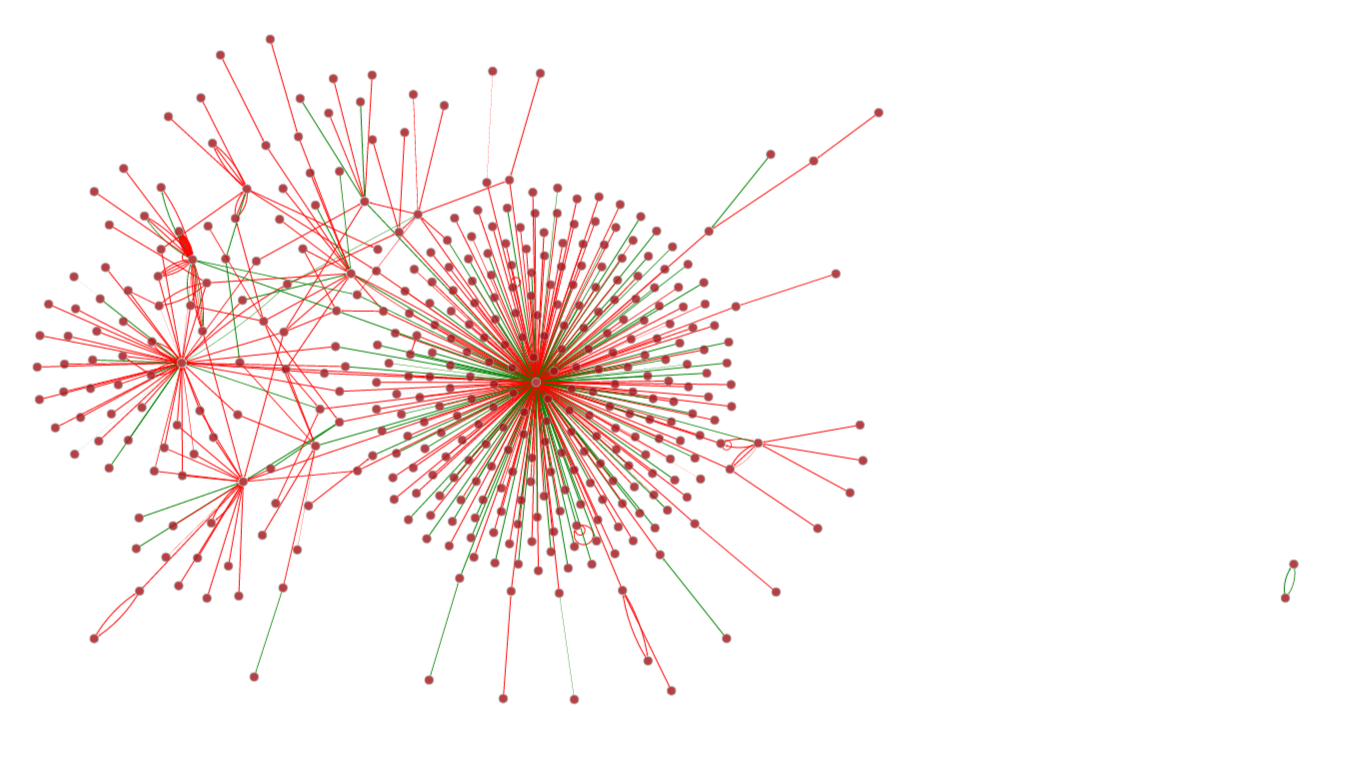
\includegraphics[width=1.1\linewidth]{img/potus_more.png}
        \caption{Graph built on previous @POTUS tweet, including \textit{Quote
        replies}}
        \label{fig:img/potus_more}
    \end{figure}
\end{frame}

\begin{frame}[c]
    \frametitle{About Twitter data (3)}
    \begin{figure}[h]
        \centering
        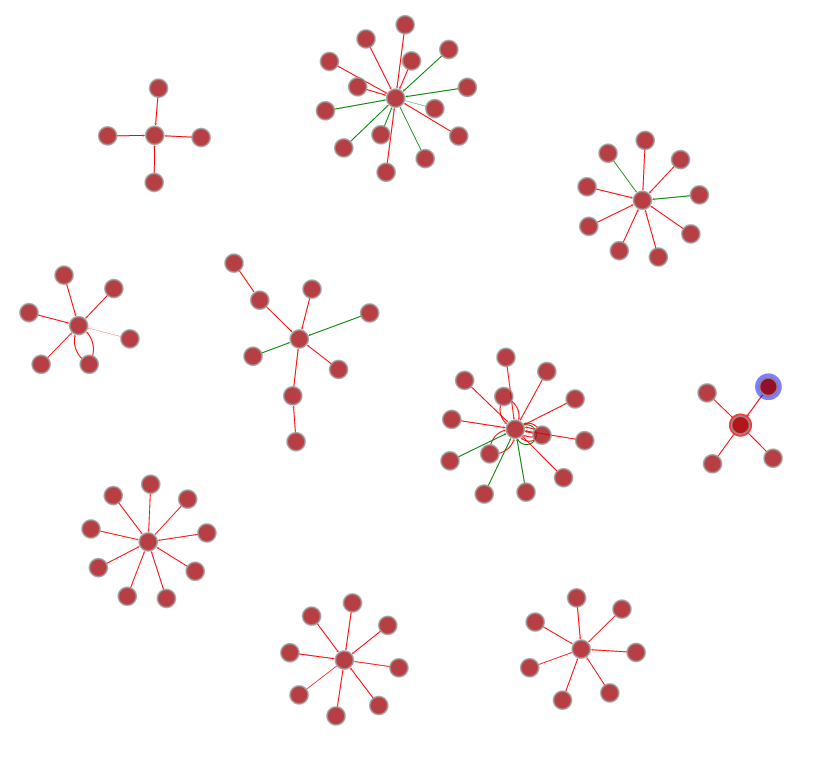
\includegraphics[width=0.7\linewidth]{img/reddit_covid_graph.png}
        \caption{Graph built on 10 statuses with > 5 replies containing "covid"}
        \label{fig:img/potus_more}
    \end{figure}
\end{frame}

\begin{frame}[c]
    \frametitle{About Reddit data (1)}
    \begin{itemize}
        \item Crossposts are few, even for most diffused posts
        \item Most of the times there are a handful of posts with around 5
            comments
    \end{itemize}

    \begin{figure}[h]
        \centering
        \begin{subfigure}[b]{0.8\textwidth}
            \begin{center}
                
\includegraphics[width=0.8\linewidth]{img/reddit_politics.png}
            \end{center}
        \end{subfigure}
    \end{figure}
\end{frame}

\begin{frame}[c]
    \frametitle{About Reddit data (2)}

    \begin{figure}[h]
        \centering
        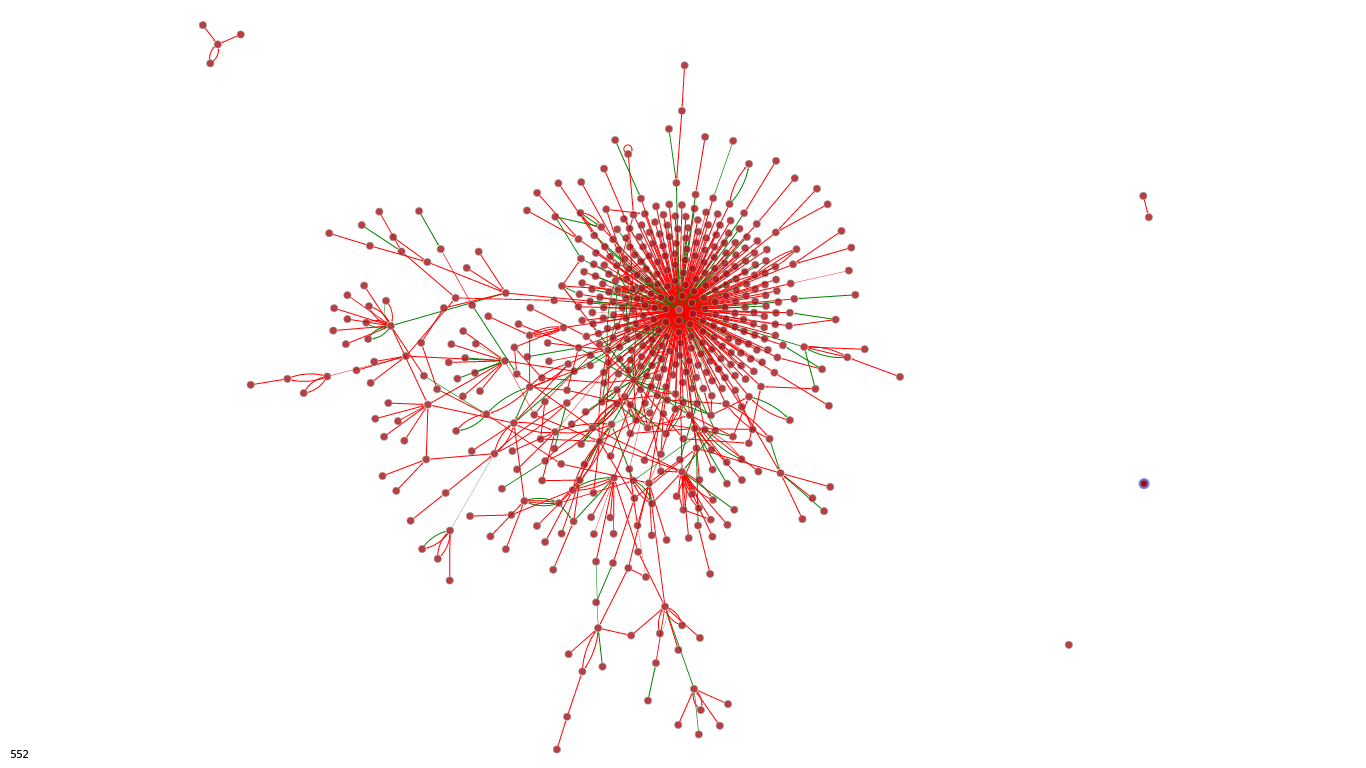
\includegraphics[width=\linewidth]{img/reddit_politics_graph.png}
        \caption{Graph built over the previous post}%
        \label{fig:img/reddit_politics_graph}
    \end{figure}
\end{frame}

\begin{frame}[c]
    \frametitle{About Reddit data (3)}

    \begin{figure}[h]
        \centering
        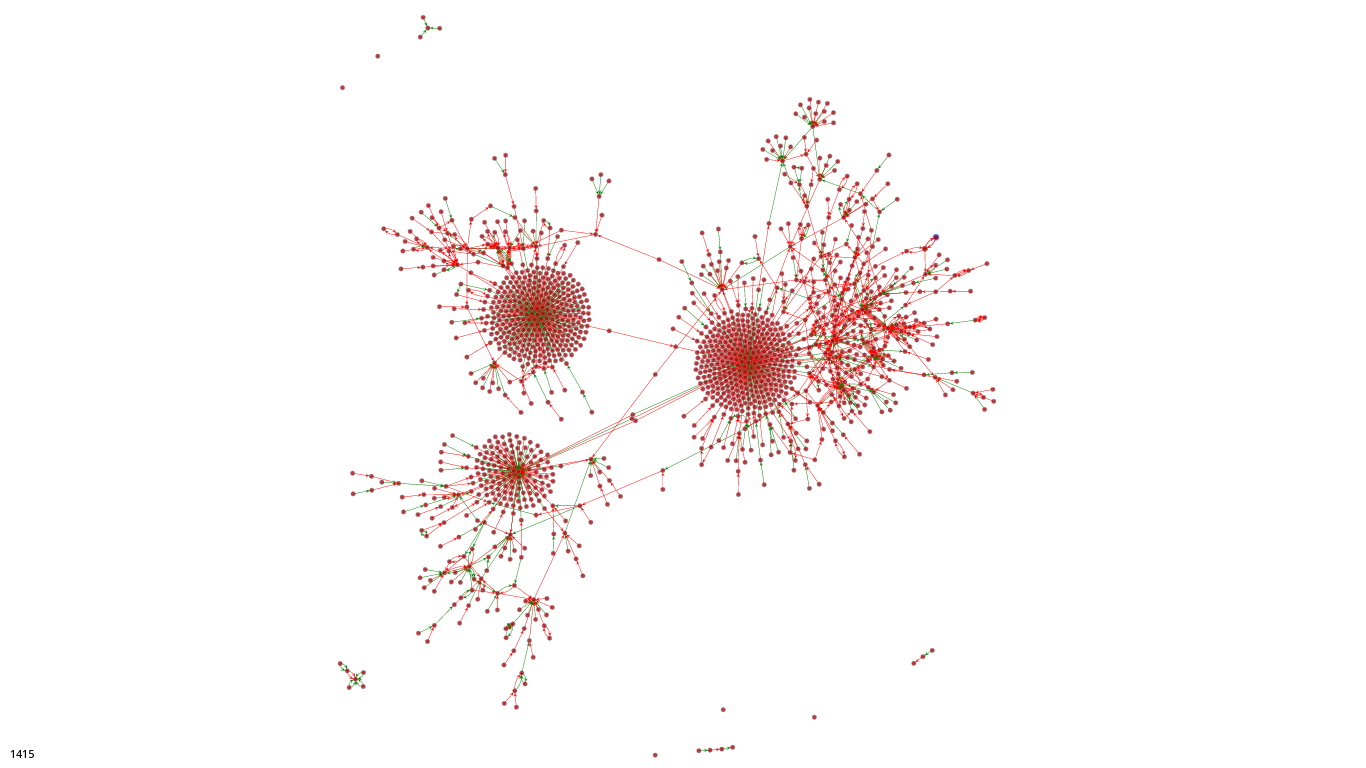
\includegraphics[width=\linewidth]{img/reddit_all_3.png}
        \caption{Graph built over 3 posts from \textit{r/all}}%
        \label{fig:img/reddit_politics_graph}
    \end{figure}
\end{frame}

\begin{frame}[c]
    \frametitle{About Reddit data (4)}

    \begin{figure}[h]
        \centering
        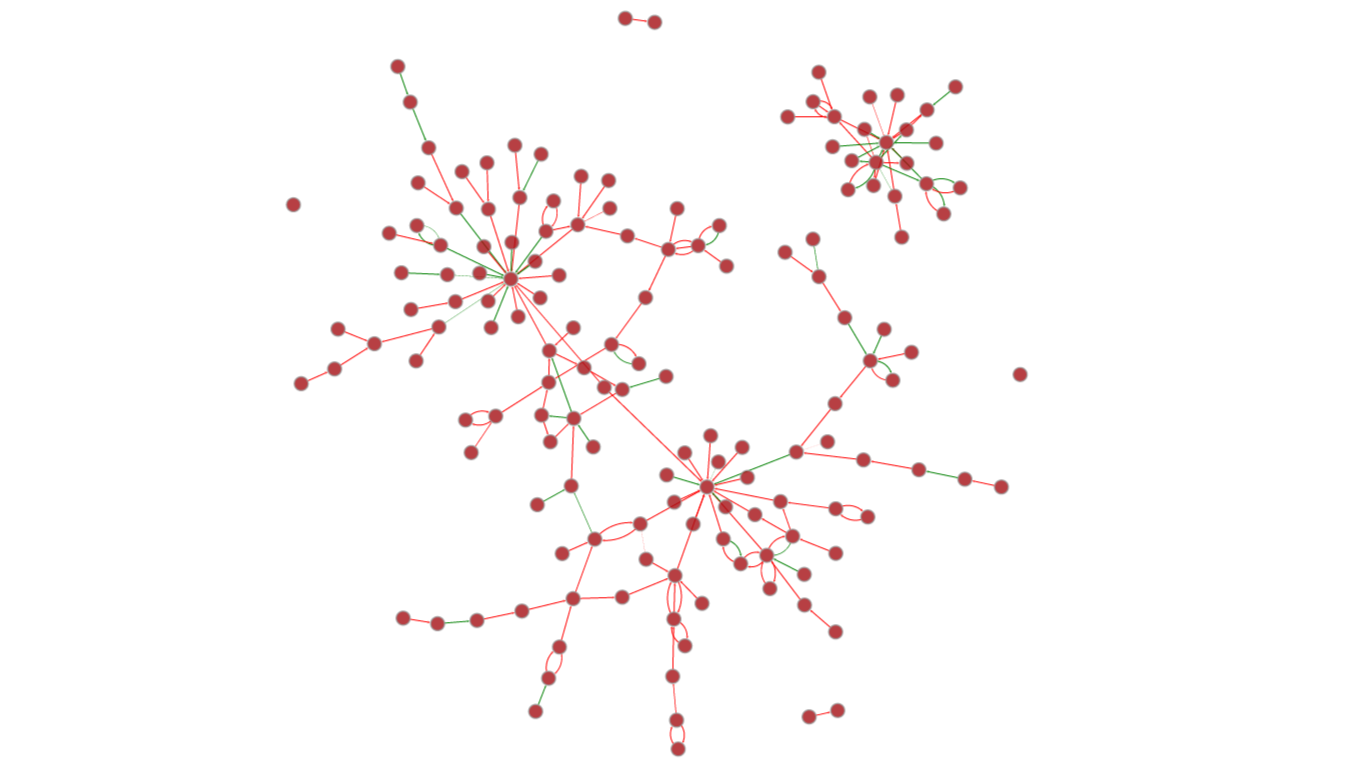
\includegraphics[width=\linewidth]{img/reddit_programming_5.png}
        \caption{Graph built over 5 posts from \textit{r/programming}}%
        \label{fig:img/reddit_politics_graph}
    \end{figure}
\end{frame}

\end{document}

